\chapter{Ancestry: how many histories, and what they hide}\label{ch:ancestry}

The first layer of generative information is the plainest: how many histories lead to an endpoint, and how the resulting uncertainty divides among the things one might want to know. This chapter proves that SELECT-II fibres are finite and nonempty, decomposes the ambiguity of an endpoint exactly into source, content, swap-class and within-class parts, works out the endpoint $72$ completely, and gives exact counts for the family $72^r$.

\section{Reverse edges and finite fibres}
For an integer $t\ge1$ write $s(t)=\prod_p p^{\lfloor v_p(t)/2\rfloor}$, where $v_p$ is the $p$-adic valuation, and $\tau(n)$ for the number of divisors of $n$.

@@prop:fibre-finite@@

By part (e) every endpoint has at least one \emph{complete} history, i.e.\ one from a squarefree source, which is why $A(t)$ is defined for every $t\ge1$ (the \emph{complete-history convention}). For fixed-source fibres $F_t(m_0)$ may be empty, and $A(t\,|\,m_0)$ is then undefined; $\log_20$ is never written.

\section{Ambiguity and its exact decomposition}
The number $A(t)=\log_2|F_t|$ is the \emph{capacity} of ancestry: for any probability distribution on a fibre of size $N$ the entropy lies between $0$ and $\log_2N$, with the maximum attained exactly by the uniform distribution (Gibbs' inequality~\cite{CoverThomas}). A real process that weighs histories non-uniformly therefore has $\Ent(W|T=t)<A(t)$, and the gap is the information the weighting adds. Let $T$ be the endpoint, $M$ the source, $Q$ the content, $C$ the swap class and $W$ the history.

@@thm:hierarchy@@
The four terms have clear meanings: $\Ent(M|T)$ is uncertainty about the seed, $\Ent(Q|M,T)$ about the multiset of operations given the seed, $\Ent(C|M,Q,T)$ about \emph{which reordering class} given seed and content, and $\Ent(W|C,T)$ is the residual order inside a class. The last is reordering ambiguity in the classical sense; the first three are structural.

@@prop:class-entropy@@

\section{The endpoint 72}
@@ex:72@@

\begin{figure}[ht]\centering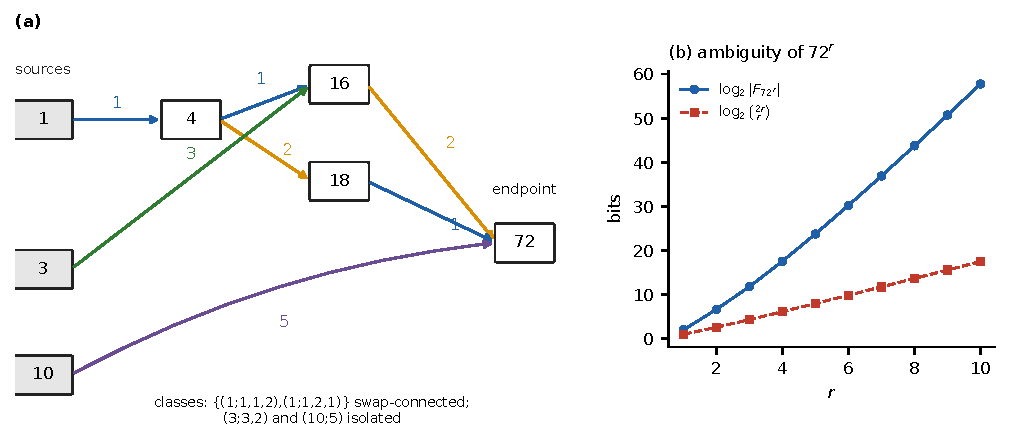
\includegraphics[width=\textwidth]{figures/fig_ancestry.pdf}
\caption{(a) The four histories of $72$ as paths of the arithmetic ancestry graph; edges carry their labels and shaded boxes are squarefree (complete) sources. The two histories from source $1$ differ by one legal swap, the labels $1,2$ at state $4$, and form a swap class; the histories from $3$ and $10$ are isolated classes. (b) Exact ambiguity $\log_2|F_{72^r}|$ against the proved lower bound $\log_2\binom{2r}{r}$ (\cref{prop:72r}).}\label{fig:ancestry}
\end{figure}

\section{Growth of ambiguity: the family \texorpdfstring{$72^r$}{72 to the r}}
How fast does ambiguity grow as the endpoint becomes richer? The simplest family is $t=72^r$, which contains a large block of independent-looking reorderings.

@@prop:72r@@
@@RAW:ch03.tex::\begin{table}[ht]\centering\small::\end{table}@@
The bound is far from sharp: at $r=10$ it gives $17.5$ bits whereas the exact value is $57.8$, because the fibre contains, besides the reorderings of $1$'s and $2$'s from source $1$, many histories through other squarefree sources and other labels. Whether $A(72^r)/r$ converges is not known.

\section{Fixed-source and complete-history ambiguity}
The two fibre conventions differ: $A(t)$ counts all complete histories, whereas $A(t\,|\,m_0)=\log_2|F_t(m_0)|$ counts those from one seed. For $72$ the complete ambiguity is $2$ bits and the fixed-source ambiguities are $1,0,0$ bits for $m_0=1,3,10$; the missing information $\Ent(M|T)=1.5$ bits is the uncertainty about the seed. In general $A(t)\ge\max_{m_0}A(t|m_0)$ and $A(t)=\log_2\sum_{m_0}|F_t(m_0)|$.

\medskip
The decomposition of \cref{thm:hierarchy} organises everything that follows: the last two terms concern histories that differ only by legal swaps, which is the geometry of \cref{ch:swaps}; the first two concern which seeds and contents are admissible, which is the arithmetic of \cref{ch:arith}.
